\documentclass[]{beamer}
\setbeamertemplate{sidebar right}{}
\setbeamertemplate{footline}{%
\hfill\usebeamertemplate***{navigation symbols}
\hspace{1cm}\insertframenumber}

\title{Robust Methods for Optical \\ Interferometry
    Images}
\subtitle[short version]{Ph.D Thesis}
\author{M. en C. Orlando Miguel Medina C\'azares}
\date{5 de Noviembre del 2015}
\institute[CIO]{Centro de Investigaciones en \'Optica}
\logo{\includegraphics[scale=0.30]{Images/cio_logo.png}}

\begin{document}

%%%%%%%%%%%%%%%%%%%%%%%%%%%%
\begin{frame}[plain]
  \maketitle
  \footnotesize{
    Asesor: Dr. Julio Estrada Rico. \\
    Co-Asesor: Dr Manuel Servin Guirado.
  }
\end{frame}
%%%%%%%%%%%%%%%%%%%%%%%%%%%%
%\begin{frame}
%\frametitle{Outline}
%\tableofcontents[part=1,pausesections]
%\end{frame}
%%%%%%%%%%%%%%%%%%%%%%%%%%%%
\begin{frame}{Algoritos de Cuadratura}
  Patr\'on de franjas:
  \begin{equation}
    I(x,y)=a(x,y)+b(x,y)cos[\phi(x,y)]
  \end{equation}
  \begin{center}
    \includegraphics[scale=0.4]{Images/Interferogram.png}
  \end{center}
\end{frame}
%%%%%%%%%%%%%%%%%%%%%%%%%%%%
\begin{frame}{Algoritos de Cuadratura}
  \includegraphics[scale=0.4]{Images/QuadratureFiltersScheme2.png}
\end{frame}
%%%%%%%%%%%%%%%%%%%%%%%%%%%%
\begin{frame}{Algoritos de Cuadratura}
\begin{center}

    \begin{eqnarray}
                      \mathcal{F}[I(x,y)] & = & I(\omega) \nonumber \\
                                                  & = & a\delta(\omega)+
                      \frac{b}{2}e^{-i \phi} \delta(\omega-\omega_0) +
                      \frac{b}{2} e^{i \phi} \delta(\omega+\omega_0)
    \end{eqnarray}
    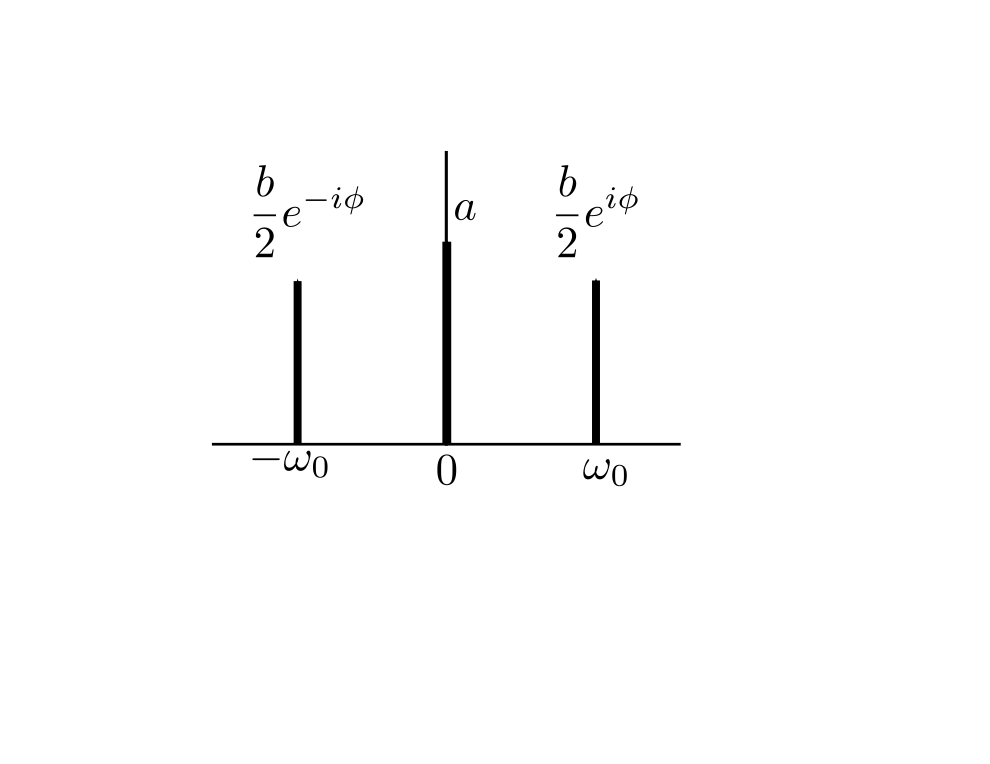
\includegraphics[scale=0.6]{Images/FourierDomine1.png}

\end{center}
\end{frame}
%%%%%%%%%%%%%%%%%%%%%%%%%%%%
\begin{frame}{Algoritos de Cuadratura}
\begin{center}

  \begin{equation}
            H(-\omega_0) =H(0) = 0, H(\omega_0) \neq 0
  \end{equation}
  \includegraphics[scale=0.6]{Images/FourierDomine2.png} 

\end{center}
\end{frame}
%%%%%%%%%%%%%%%%%%%%%%%%%%%%
\begin{frame}{Algoritos de Cuadratura}
\begin{center}

    \begin{equation}
             I(\omega) H(\omega) = \frac{b}{2}exp[i \phi]
     \end{equation}
     \includegraphics[scale=0.6]{Images/FourierDomine3.png}

  \end{center}
\end{frame}
%%%%%%%%%%%%%%%%%%%%%%%%%%%%
\begin{frame}{Algoritmos de Cuadratura}
\begin{center}

  \begin{equation}
    \hat \phi=atan\bigg[ \frac{ Im\{\frac{b}{2}exp[i \phi]\} }{
      Re\{\frac{b}{2}exp[i \phi]\} } \bigg]
  \end{equation}
  \includegraphics[scale=0.6]{Images/wPhase.pdf}

\end{center}
\end{frame}
%%%%%%%%%%%%%%%%%%%%%%%%%%%%
\begin{frame}{Filtros Regularizados}

\end{frame}
%%%%%%%%%%%%%%%%%%%%%%%%%%%%

\end{document}